\documentclass[11pt]{article}

\usepackage{booktabs}
\usepackage{dcolumn} 
\usepackage{epstopdf}
\usepackage{fourier}
\usepackage{fullpage}
\usepackage{graphicx}
\usepackage{hyperref}
\usepackage{longtable} 
\usepackage{natbib}
\usepackage{rotating}
\usepackage{tabularx}
\usepackage{amsmath}
\usepackage{threeparttable} 
% \usepackage{algorithmic} 
% \usepackage{algorithm2e}

\hypersetup{
  colorlinks = TRUE,
  citecolor=blue,
  linkcolor=red,
  urlcolor=black
}

\newcommand{\starlanguage}{Significance indicators: $p \le 0.05:*$,
  .$p \le 0.01:**$ and $p \le .001:***$.} 

% TO DO 

% Ask workers for age, gender, income & employment status? 
% Validate against Google consumer surveys 
% Check against variance in that occupation---is greater pct error driven by greater variance? 

%% The sample of workers answering questions on MTurk. 
%% If a pattern or causal effect exists in one population, there is always a question of generalizability. 
%% What if the sample of respondents is just a sample of low-wage workers? 
%% - We can ask workers for their incomes 
%% - We can show in the literature that this is not a particularly biased group 
%% - We can use Google Survey, a nationally representative sample, to adjust 
%% What if high-way jobs are just less common? Controlling for the total employment in that category does not make the effect go away. 
%% What if the hourly/annual salary throws things off? 
%% Do high-way jobs just have more variance? 
%% Was the hourly range top-coded? We started using different binnings that the top, which mechanically reduces predictive accuracy.  
%% Should the panel estimates have clustered standard errors? 
%% Is the BLS 'major' category the right one? The ``Managerial, Other'' type occupations are not really adding much to the analysis. 
%% Turn both knowledge measures into Likert scales 

%% Future work 
%% Wage profile tenure 
%% Link up with representative data 
%% Perhaps one could sample some vacancies as a ``stake in the ground.'' 

%Even when controlling for social knowledge, error percentages increase with the actual wage of the occupation. 
% Preview results 
% Respondent knowledge appears segmented, in that workers 
%% The focus on the analysis was to:
%% -characterize performance and see whether the ``wisdom of crowds'' hypotheses holds regarding occupations 
%% -find poorly labeled occupations in the BLS/OES 
%% -see what occupations are misperceived. 
%% -see how total employment and social knowledge mediate performance in estimating hourly wages 
%% -test whether social knowledge is ``segmented'' by wage  
%% - Idea: break bands, with four drop downs into (0 - 25)(26-50)(51 - 75)(76 - 100)
%% Why are physicains and surgeons ``off'' - is it top-coded? 

% Questions: 
% 1) Are log wages homoscedastic wrt to standard errors? 

\newcommand{\numRaters}{127}
\newcommand{\numOccupations}{99}
 

\begin{document} 

\title{Folk Knowledge of the World of Work: \\ Quantifying Perceptions of Occupational Attributes}

\date{\today}

\author{John J. Horton \\ Leonard N. Stern School of Business, New
  York University\footnote{Author contact information, datasets and
    code are currently or will be available at
    \href{http://www.john-joseph-horton.com/}{http://www.john-joseph-horton.com/}. 
    Thanks to Alex Gedranovich for excellent research assistance. 
} }
\maketitle

\begin{abstract}
\noindent  
A sample of labor market participants were asked to estimate the wage and projected employment growth for a selection of BLS occupations; they also reported whether they knew anyone working in that occupation. 
``Social'' knowledge about an occupation---knowing someone working in that occupation---is associated with more accurate predictions of both the wages and future employment trends in that occupation, even when controlling for both the respondent and the occupation (respondents were asked about multiple occupations).  
At the occupation level, wage estimation and employment trend prediction errors are decreasing in the fraction of the population employed in that occupation.  
Respondents systematically underestimate the wages of higher-wage occupations, even when controlling for social knowledge. 
Managerial occupations are particularly pronounced outliers, with respondents strongly under-estimating the returns to being a manager.   
Respondent social knowledge is stratified by occupational hourly wage, with respondents knowing people in high-wage or low-wage occupations, but generally not both.  
\newline 
\newline 
\noindent JEL J01, J24, J3
\end{abstract} 

\section{Introduction}
To plan their careers, labor market participants should know what various occupations pay and the future prospects of those occupations. 
Misinformation about the current and future prospects of different careers could lead to poorly considered human capital decisions. 
This study assess the accuracy of career information held by a convenience sample of the US population---albeit one that is similar to the sub-population for whom accurate labor market information is most consequential. 
The main focus of the paper is on how occupational and individual characteristics mediate estimation accuracy. 

For the 99 US occupations (as measured by the May 2013 OES) with the greatest employment totals, respondents from Amazon Mechanical Turk were asked whether: 
(1) they knew what the occupation consisted of 
(2) how many people they knew who held that occupation, if any,  
(3) their estimate of the hourly wage for that occupation
and (4) whether in the future, wages and employment in that occupation would rise, fall or stay the same. 
There were no incentives for correct answers and the short time most workers spend on any tasks suggests they were not performing research. 

Excluding some notable exceptions, respondents---at least collectively---demonstrated that they possessed substantial labor market knowledge: 
respondent mean estimates of hourly wages explain over 70\% of the actual variation in wages.
However, the residual variation was not idiosyncratic.  
Respondent predictions become less accurate the higher the wage for the occupation.
In particular, respondents underestimate the wages of higher wage jobs. 
This is not simply because higher wage jobs are less common or that workers know fewer people with those occupations: 
controlling for the total employment in that occupation and whether the worker knows someone in that occupation, the negative relationship still exists. 

Using fixed effects for both the worker and occupation, we show that knowing someone with a particulr occupation---``social knowledge''---reduces wage prediction error. 
Presumably wage information is just one dimension of occupational knowledge that gets passed along through social connections. 
If first-hand social knowledge is an important disseminator of labor market information, it suggests that isolated individuals exposed to a narrow slice of occupational possibilities could be at a labor market disadvantage. 
Social knowledge itself displays an interesting U-shaped pattern: 
workers know people with low wage jobs and high wage jobs, but know far fewer people in middle wage occupations. 
Respondent knowledge is also stratified by occupational income. 
Workers do not know about random subsets of occupations, but instead, knowing more high occupations makes it more likely that the respondent will know some other high wage occupation. 

One concern with this study is that results from convenience samples do not necessarily generalize to the larger population. 
Even if they are representative, there is the unavoidable selection concern borne from the fact that the sample was recruited from an online marketplace. 
However, convience samples---beyond just being convenient---can given credible results for certain kinds of questions, particularly those trying to detect correlations.
Laboratory economics experiments also use convenience samples under a similar logic. 
The epistemological justification in laboratory experiments that that even if ``means'' do not necessarily generalize---say the proportion of people in college or the magnitude of some treatment effect---correlations and directional relationships are more likely to hold generally.\footnote{ 
For example, volunteers for a clinical trial presumably do not have hypertension at the same rate as the population, but if some drug can reduce levels of hypertension in a clinical trial, we suspect that directinal effect would also hold in the population.}
While not guaranteed to be true, it does make findings about 

One result that is both important and seemingly sensitive to the choice in population is the declining accuracy with increased wages. 
It is true that workers on Mechnical Turk are unrepresentative, in that they have lower than average wages (and tend to be younger), this is an advantage of this sample. 
However, given the motivation of the paper---assessing the accuracy of labor market information for would-be labor market participants faced with human capital decisions---this relative povery and youthfulness of the MTurk population is a plus. 

If the patterns discovered here generalize, the good news is that they might be readily fixed: 
several studies have highlighted the powerful effects obtainable from purely informational interventions (e.g., \cite{jensen2010perceived}, \cite{dupas2009teenagers}, \cite{card2010inequality}).\footnote{The connection between labor market information and allocative efficiency was in part the motivation for the Knowledge of the World of Work (KWW) test, which was briefly included in the NLSY \citep{kohen1975}.}

%% Granovetter---weak ties. 
%% Some evidence for the Social learning hypotheses.  

\cite{rees1966information} 
\cite{stigler1962information}
\cite{hlavac2013} for stargazer. 
\cite{ward1992} 
\cite{pallais2013referential} 
\cite{burks2013value} 
\cite{betts1996students} 
\cite{webbink2004} 
\cite{dominitz1996} 

\section{Data collection and description} 
A total of \N\, respondents participated in th survey. 
The respondents on average gaves responses for TK occupations; the median count of occupations was TK.  
Each occupation was estimated by TK different respondents. 
The actual survey interface presented to respondents in shown in Appendix A, Figure~\ref{fig:survey}. 
The heading labeled would show the BLS occupation title. 

For the social knowledge measure, respondents were asked how many individuals they knew in an occupation. 
The choices were $0$, $1$, $3-10$ and more than $10$. 
To construct a social index, these bins were coded as 0, 1, 2 and 3, respectively and then normalized. 

\section{Empirical Results}

Our primary concern is whether respondents have correct beliefs about wages. 
Figure~\ref{fig:prediction_scatter} is a scatter plot of the log actual wages (y-axis) versus the mean of log predicted wages (x-axis) for each occupation. 
Deviations from the 45 degree line indicate prediction errors. 
Outliers---both positive and negative---are labeled with the occupation title.  
There are two notable features of the data clearly illustrated by the the plot. 
First, it seems that workers systematically underestimate the wages of occupations at the high end of the distribution.  
Second, many of the extreme outliers are under-estimates of the wages of managerial occupations. 
The only occupation that workers substantially over-estimate is the home health aide category---perhaps becaus of a mistaken belief that this is the nursing occupation.

\begin{figure}
\caption{Perceived hourly wages versus actual hourly wages \label{fig:prediction_scatter}} 
\centering 
\begin{minipage}{0.90 \linewidth}
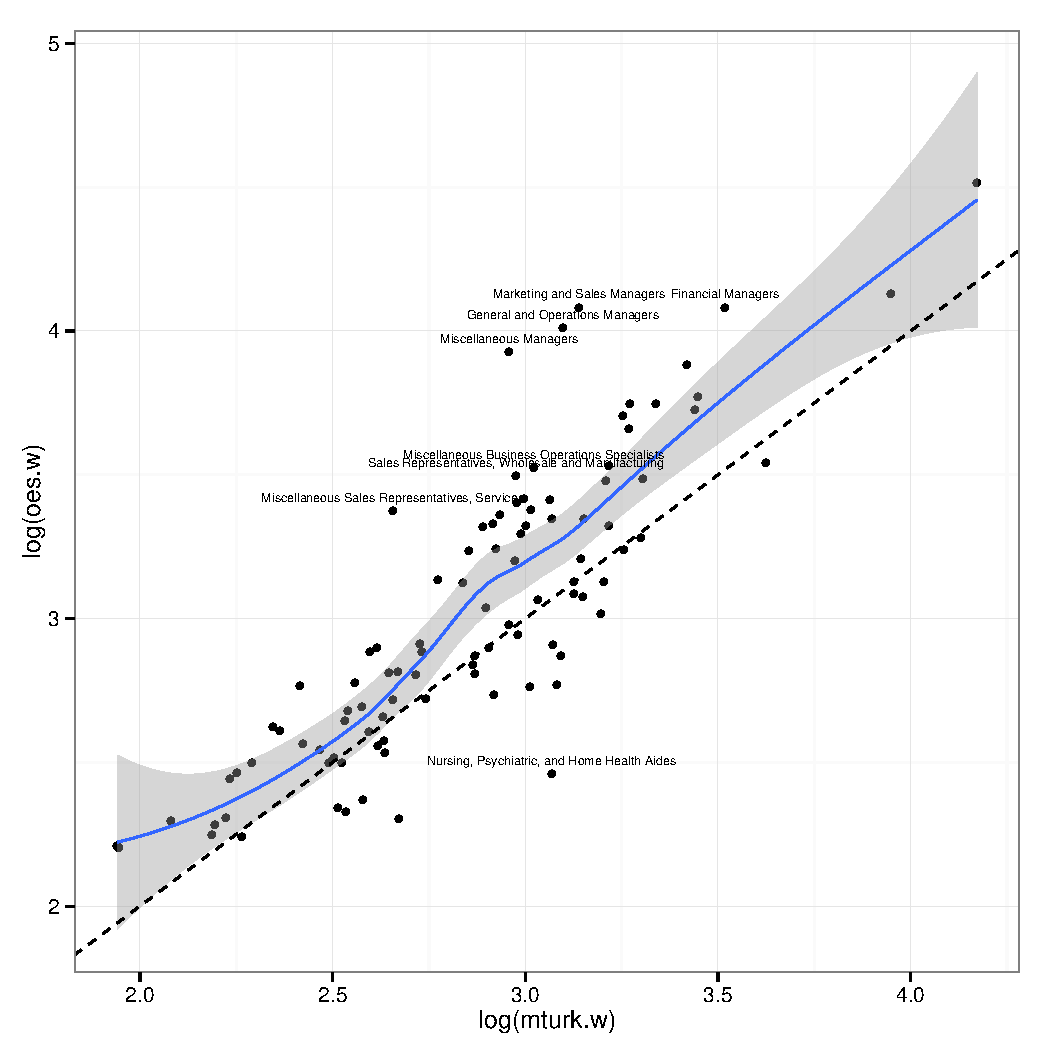
\includegraphics[width = \linewidth]{./plots/predicted_v_actual.pdf} 
\\
\emph{Notes:} This plot shows the actual log mean wage versus the mean log wages versus predicted wages.  
\end{minipage}  
\end{figure} 

To explore the apparent systematic under-estimation of wages, in Figure~\ref{fig:by_occupation_boxplots} we plot the distribution of individual respondent log wage estimates for each occupation as a box plot. 
The actual mean and median wage for each occupation are shown as squares TK and triangles TK, respectively. 
Occupations are ordered by mean wage, from highest to lowest. 
By comparing the median of the boxplot to the actual median, we can see the tendency of respondents to systematically underestimate the wages at the high end of the distribution. 
The bias does not seem to be driven by high or low outliers that pull the mean away from the truth. 

\begin{figure}
\caption{Distributions of respondent hourly wage perceptions by occupation \label{fig:by_occupation_boxplots}} 
\centering 
\begin{minipage}{0.90\linewidth}
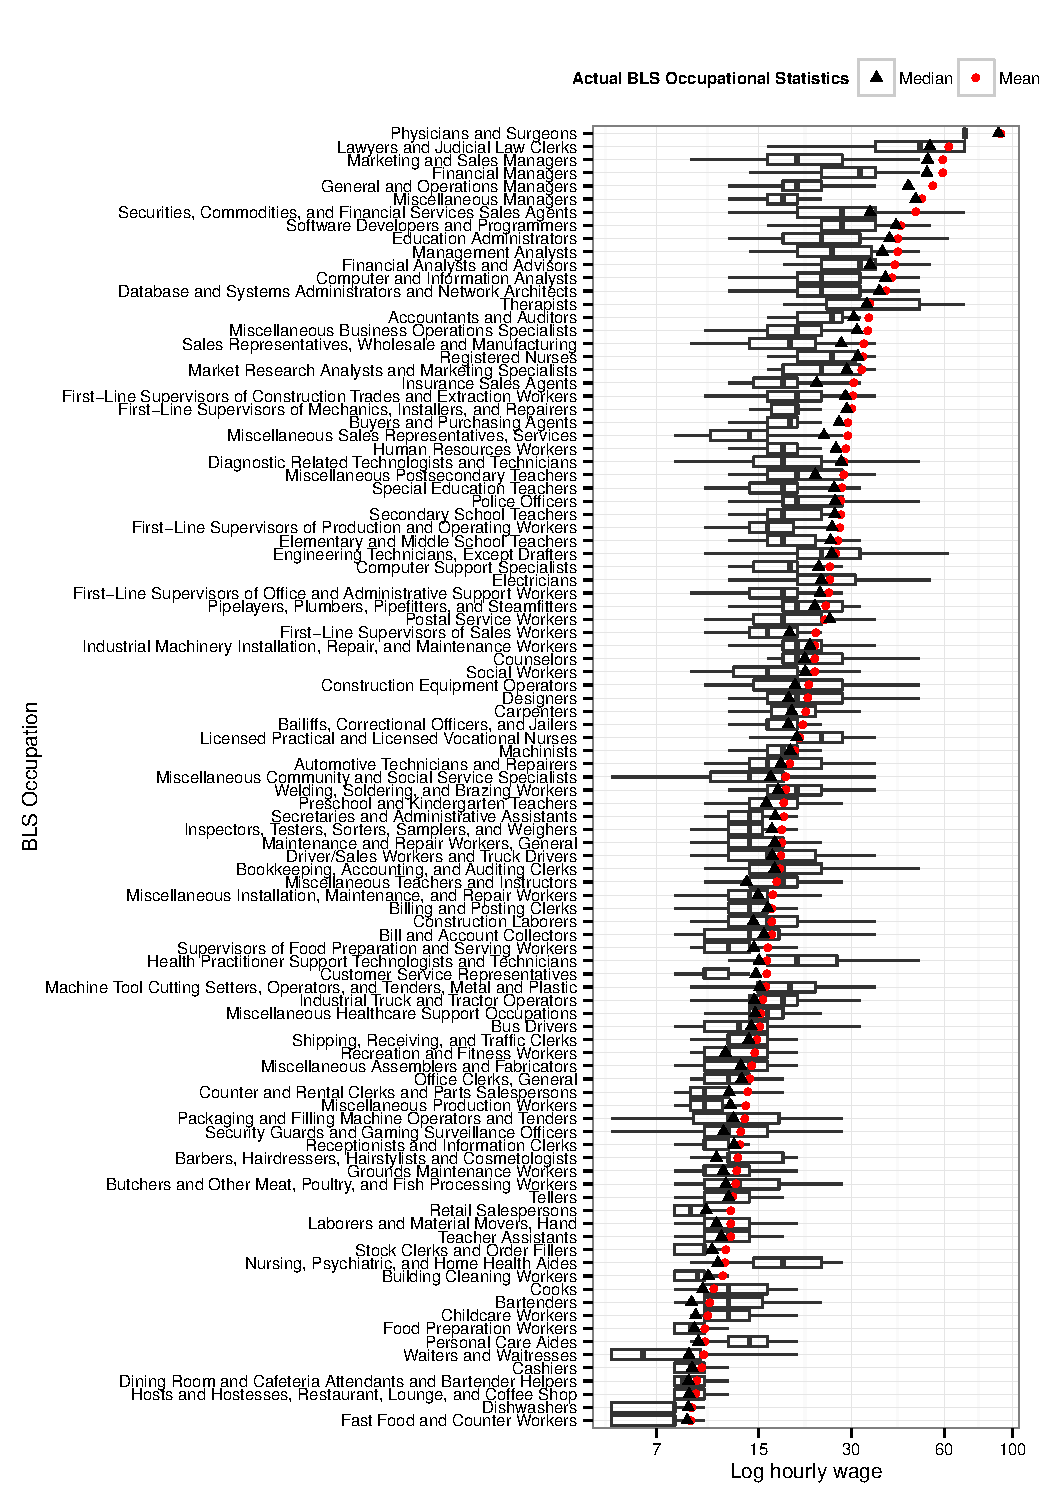
\includegraphics[width = \linewidth]{./plots/box_plots_by_occupation.pdf} 
\emph{Notes:} Boxplots of the respondent wage predictions are shown for each occupation.
The actual mean is shown in TK, while the actual median is shown in TK.  
\end{minipage}
\end{figure} 

\subsection{Determinants of the occupational knowledge and accuracy} 

Table~\ref{tab:occupation_accuracy} reports several regression where the outcome variable is the MSE in prediction, in log points. 
In Column~(1), we can see, unsurprisingly, that prediction errors are decreasing in the total employment in that population. 
Column~(2) adds as a predictor and indicator for whther the respondent knows that the job consists of. 
This is also negative, as expected, and lowers the employment coefficient.  
Column~(3) adds the social index predictor, which is negative (albeit not significant) lowers the employment and job knowledge coefficients. 
Finally, in Column~(4), we add the log mean hourly wage. 
It is strongly positive---consistent with our graphical evidence---and it also flips the sign of the employment coefficient.  
It also dramatically increases the adjusted $R^2$ of the regression. 
In the data, actual occupational wages and employment share have a strong negative correlation, which this sign-reversal reflects. 


% Table created by stargazer v.4.5.3 by Marek Hlavac, Harvard University. E-mail: hlavac at fas.harvard.edu
% Date and time: Tue, Dec 17, 2013 - 05:02:38 AM
\begin{table}[!htbp] \centering 
  \caption{Occupation attributes and worker accuracy} 
  \label{tab:occupation_accuracy} 
\begin{tabular}{@{\extracolsep{5pt}}lcccccc} 
\\[-1.8ex]\hline 
\hline \\[-1.8ex] 
 & \multicolumn{6}{c}{\textit{Dependent variable:}} \\ 
\cline{2-7} 
\\[-1.8ex] & \multicolumn{3}{c}{mse.wage} & \multicolumn{3}{c}{mse.v.trend} \\ 
\\[-1.8ex] & (1) & (2) & (3) & (4) & (5) & (6)\\ 
\hline \\[-1.8ex] 
 log(tot.emp) & $-$0.088 & 0.064 & 0.480 & 0.024 & 0.021 & $-$0.016 \\ 
  & (0.081) & (0.065) & (0.381) & (0.043) & (0.045) & (0.265) \\ 
  & & & & & & \\ 
 log(avg.wage) &  & 0.720$^{***}$ & 2.698 &  & $-$0.012 & $-$0.187 \\ 
  &  & (0.088) & (1.788) &  & (0.061) & (1.242) \\ 
  & & & & & & \\ 
 log(tot.emp):log(avg.wage) &  &  & $-$0.147 &  &  & 0.013 \\ 
  &  &  & (0.132) &  &  & (0.092) \\ 
  & & & & & & \\ 
 Constant & 1.196 & $-$3.041$^{**}$ & $-$8.667 & 0.413 & 0.486 & 0.983 \\ 
  & (1.104) & (0.995) & (5.175) & (0.584) & (0.687) & (3.595) \\ 
  & & & & & & \\ 
\hline \\[-1.8ex] 
Observations & 99 & 99 & 99 & 99 & 99 & 99 \\ 
R$^{2}$ & 0.012 & 0.419 & 0.427 & 0.003 & 0.004 & 0.004 \\ 
\hline 
\hline \\[-1.8ex] 
\multicolumn{5}{p{0.80 \linewidth}}{
\emph{Notes:} This table reports descriptive regressions where the
depdendent variable is the MSE in respondent log wage prediction and the
 independent variables are the effects of social and general knowledge on a
respondent's prediction error, while controlling for worker and
occupation specfic effects. In Columns (1) and (2), the dependent
variable is MSE in wage prediction, while in Columns (3) and (4), the
dependent variable is an indicator for incorrectly predicting the
direction of employment growth in that occupation. Columns (1) and (3)
use worker and occupation fixed effects, with standard errors
clustered at the level of the respondent (the more converative
clustering choice), while in Columns (2) and (3), a multi-level model
with respondent and title random effects are used. \starlanguage 
}\end{tabular} 
\end{table} 


Given the strong effects that wage has on predictive accuracy, a natural question is how social knowledge and job knowledge vary with wage. 
Figure~\ref{fig:knowledge_by_wage} plots the fraction of respondents reporting that they know what an occupation is (in TK) and whether they know someone with that occupation (in TK), binned by hourly wage. 
A clear U-shaped pattern is apparent: respondnents know more---both socially and substantiively---about low- and high-wage occupations, but less about the middle. 
This cuts against the idea that the population of respondents---which generally have low wages---simply does not know anyone at the top of the distribution. 
While the reason for the pattern in unclear, it could reflect frequent exposure to service occupations---both high and low-end---but relatively little exposure to managerial, trade and operational occupations that, as a matter of course, do not interact with individual consumers.  
Individuals are exposed regularly to low-wage jobs like waitresses and custodial workers and high-wage but professional jobs like doctors, dentists and lawyers, but they have little day-to-day experience with various managers, technical specialists, trade persons etc. that fill up the bulk of the mid-tier occupations. 

\begin{figure}
\caption{Hourly wage and occupational knowledge \label{fig:knowledge_by_wage}} 
\centering
\begin{minipage}{0.90 \linewidth}
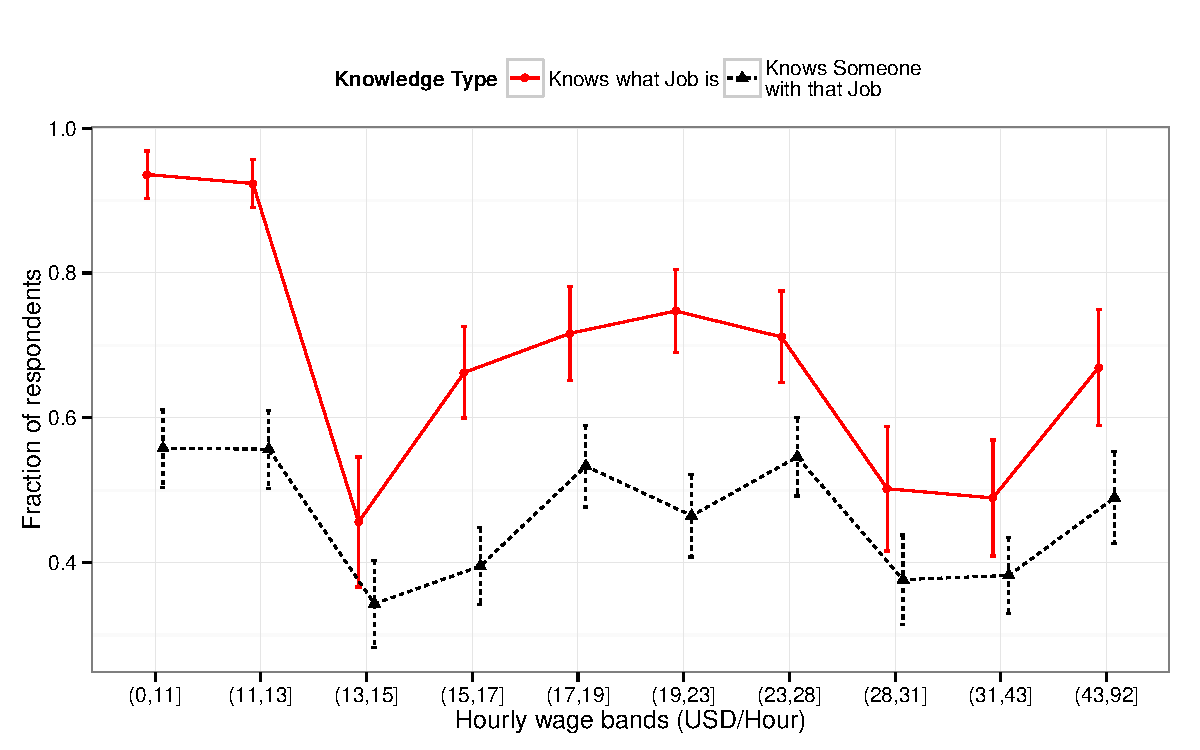
\includegraphics[width = \linewidth]{./plots/knowledge_by_wage.pdf}
\\
\emph{Notes:} This figure shows the mean fraction of respondents either knowing someone or knowing what an occupation consists of, by hourly wage bands. 
\end{minipage}  
\end{figure} 

\subsection{Determinants of individual performance} 
In Table~\ref{tab:panel_prediction}, Column~(1), we use the log points outcome measure, while in Column~(2) we use the percentage outcome measure. 
Both regressions are fixed effect regressions, with fixed effects for both the respondnent and the occupation.  
We can see that social knowledge is associated with lower prediction error---in both specifications, social knowledge is negative and significant. 
Controlling for both the individual and the worker lets us isolate the effect of social knowledge. 
It is not the case---as it would be in cross-sections---that individuals with lots of social knowledge have reduced error rates or that occupations that are well-known socially also have little error. 
While social knowledge is of course not as good as randomly assigned---reverse causation---say having accurate beliefs about a particular occupation causes one to have friends with that occupation---seems implausible. 

% 
% Table created by stargazer v.4.5.3 by Marek Hlavac, Harvard University. E-mail: hlavac at fas.harvard.edu
% Date and time: Sat, Dec 14, 2013 - 07:27:59 AM
\begin{table}[!htbp] \centering 
  \caption{Fixed effects estimation of social knowledge and job knowledge on MSE in log hourly wage predictions} 
  \label{tab:panel_prediction} 
\begin{tabular}{@{\extracolsep{5pt}}lcc} 
\\[-1.8ex]\hline 
\hline \\[-1.8ex] 
 & \multicolumn{2}{c}{\textit{Dependent variable:}} \\ 
\cline{2-3} 
 & MSE of log points & MSE Log wage pct \\ 
\\[-1.8ex] & (1) & (2)\\ 
\hline \\[-1.8ex] 
 Social index & $-$0.039$^{*}$ & $-$0.036$^{*}$ \\ 
  & (0.017) & (0.017) \\ 
  & & \\ 
 Job Knowledge Index & $-$0.022 & $-$0.023 \\ 
  & (0.034) & (0.036) \\ 
  & & \\ 
\hline \\[-1.8ex] 
Observations & 2,951 & 2,951 \\ 
R$^{2}$ & 0.003 & 0.002 \\ 
Adjusted R$^{2}$ & 0.003 & 0.002 \\ 
F Statistic (df = 2; 2850) & 4.014$^{*}$ & 2.958 \\ 
\hline 
\hline \\[-1.8ex] 
\textit{Note:}  & \multicolumn{2}{l}{$^{*}$p$<$0.05; $^{**}$p$<$0.01; $^{***}$p$<$0.001} \\ 
 & \multicolumn{2}{l}{Here are some notes} \\ 
\normalsize 
\end{tabular} 
\end{table} 
  

%\begin{table}[htbp]\centering
\def\sym#1{\ifmmode^{#1}\else\(^{#1}\)\fi}
\caption{Social Knowledge and Labor Market Information Accuracy}
\begin{tabular}{l*{2}{c}}
\hline\hline
            &\multicolumn{1}{c}{(1)}         &\multicolumn{1}{c}{(2)}         \\
            &       error         &       Error         \\
\hline
Social Index&      -0.008         &      -0.047\sym{**} \\
            &     (0.006)         &     (0.017)         \\
Job Knowledge Index&      -0.001         &      -0.025         \\
            &     (0.011)         &     (0.031)         \\
\hline
\(N\)       &        2952         &        2952         \\
\hline\hline
\multicolumn{3}{l}{\footnotesize Standard errors in parentheses}\\
\multicolumn{3}{l}{\footnotesize \sym{*} \(p<0.05\), \sym{**} \(p<0.01\), \sym{***} \(p<0.001\)}\\
\end{tabular}
\end{table}
  



% Table created by stargazer v.5.1 by Marek Hlavac, Harvard University. E-mail: hlavac at fas.harvard.edu
% Date and time: Mon, Mar 02, 2015 - 03:31:23 PM
\begin{table}[!htbp] \centering 
  \caption{Social and errors in occupational wage and employment trajectories} 
  \label{tab:fe_errors} 
\begin{tabular}{@{\extracolsep{5pt}}lcc} 
\\[-1.8ex]\hline 
\hline \\[-1.8ex] 
 & \multicolumn{2}{c}{\textit{Dependent variable:}} \\ 
\cline{2-3} 
 & Wage Error & Employment Trend Error \\ 
\\[-1.8ex] & (1) & (2)\\ 
\hline \\[-1.8ex] 
 Social Knowledge Index & $-$0.030 & $-$0.054$^{**}$ \\ 
  & (0.025) & (0.019) \\ 
  & & \\ 
\hline \\[-1.8ex] 
Respondent FE & Yes & Yes \\ 
Occupation FE & Yes & Yes \\ 
Observations & 1,898 & 1,898 \\ 
R$^{2}$ & 0.373 & 0.327 \\ 
Adjusted R$^{2}$ & 0.304 & 0.252 \\ 
\hline 
\hline \\[-1.8ex] 
\end{tabular}
\\
\begin{minipage}{0.95 \textwidth}
{\footnotesize \emph{Notes:} This table reports the effects of social and general knowledge on a
respondent's prediction error, while controlling for worker and
occupation specfic effects. In Columns (1) the dependent
variable is MSE in wage prediction, while in Column (2), the
dependent variable is an indicator for incorrectly predicting the
direction of employment growth in that occupation. \starlanguage }
\end{minipage}
\end{table}



\subsection{Stratification of knowledge} 

A important question is whether workers are stratified in their knowledge about wages. 
If workers only know about wages ``locally'' they might be stuck in a kind of trap, unwilling to make substantial human capital investments without more certainty about the reward.  
This possibility is even more important if drop-offs in knowledge are ``steep'' and if ignorance is increaes in wages---both patterns that exist in the survey.  

We can test partially test this stratication proposition using our data, by seeing whether, for each occupation, social knowledge is predicted by the mean wages of the other occupations for which the worker claimed to have social knowledge. 
To fix ideas, consider an occupation, $j$. 
For that occupation, have an collection of individual wage estimates, $\hat{w}_{ij}$. 
For this measure, we compute $\bar{w}^S_{-j}$, which is the mean wage of other occupations for which the worker had social knowledge.  
We then regress: 
\begin{align} \label{eq:cluster}
Pr\{S_i = 1\} = \alpha + \beta \log w_i + \gamma \log \bar{w}^S_{-i} + \delta \log w_i \times \log \bar{w}^S_{-i} + \epsilon_{ij} 
\end{align} 

Table~\ref{tab:clustering}, we estimate Equation~\ref{eq:cluster}. 
As all our previous results have indicated, knowledge is decreasing in the wage of the occupation: $\hat{\beta}$ is negative. 
Consistent with the stratification hypotheses, the coefficient on the acutal wage and the social knowedge wage is positive, or $\hat{\delta} > 0$. 
Respondents that reported knowing people in higher-wage occupation where more likely to know someone in the $i$th occupation if the $i$th occupation was itself higher-wage. 

%%%%%%%%%%%%%%%%%%%%%%%%%%%%%%%%%%%%%%%%%%%%%%%%%%%%%%%%%%%%%%%%%%%%%%%%%%%%%%%%%%%%%%%%%%%%%%%%%%%%%%%%%%%%%%%%%%%%%%%%%%%%%%%%%%%%%%%%%%%%%%
%
% Calls:
% (1):  lm(formula = I(social > -2) ~ log(actual.mean.wage) * mean.wage.others.social + log(tot.emp), data = by.worker.df) 
% (2):  lmer(formula = I(social > -2) ~ log(actual.mean.wage) * mean.wage.others.social + log(tot.emp) + (1 | WorkerId), data = by.worker.df) 
% (3):  lmer(formula = I(social > -2) ~ log(actual.mean.wage) * mean.wage.others.social + (1 | WorkerId) + (1 | title), data = by.worker.df) 
%
%%%%%%%%%%%%%%%%%%%%%%%%%%%%%%%%%%%%%%%%%%%%%%%%%%%%%%%%%%%%%%%%%%%%%%%%%%%%%%%%%%%%%%%%%%%%%%%%%%%%%%%%%%%%%%%%%%%%%%%%%%%%%%%%%%%%%%%%%%%%%%
\begin{tabular}{lcD{.}{.}{7}cD{.}{.}{7}cD{.}{.}{7}}
\toprule
&&\multicolumn{1}{c}{(1)} && \multicolumn{1}{c}{(2)} && \multicolumn{1}{c}{(3)}\\
\midrule
(Intercept)                                             &  &  3.574^{***} &&  2.699^{**}  &&  4.880^{***}\\
                                                        &  &  (1.015)     &&  (0.977)     &&  (0.929)    \\
log(actual.mean.wage)                                   &  & -1.510^{***} && -1.244^{***} && -1.390^{***}\\
                                                        &  &  (0.327)     &&  (0.306)     &&  (0.296)    \\
mean.wage.others.social                                 &  & -1.626^{***} && -1.318^{***} && -1.406^{***}\\
                                                        &  &  (0.332)     &&  (0.320)     &&  (0.307)    \\
log(tot.emp)                                            &  &  0.131^{***} &&  0.131^{***} &&             \\
                                                        &  &  (0.015)     &&  (0.014)     &&             \\
log(actual.mean.wage) $\times$ mean.wage.others.social &  &  0.504^{***} &&  0.415^{***} &&  0.447^{***}\\
                                                        &  &  (0.109)     &&  (0.102)     &&  (0.098)    \\
Var((Intercept)|WorkerId)                               &  &              &&   0.045      &&   0.040     \\
                                                        &  &              &&              &&             \\
Var(|Residual)                                          &  &              &&   0.198      &&   0.179     \\
                                                        &  &              &&              &&             \\
Var((Intercept)|title)                                  &  &              &&              &&   0.027     \\
                                                        &  &              &&              &&             \\
\midrule
R-squared                                               &  &      0.040   &&              &&             \\
adj. R-squared                                          &  &      0.039   &&              &&             \\
sigma                                                   &  &      0.489   &&              &&             \\
F                                                       &  &     26.252   &&              &&             \\
p                                                       &  &      0.000   &&              &&             \\
Log-likelihood                                          &  &  -1754.623   &&  -1609.371   &&  -1555.602  \\
Deviance                                                &  &    596.067   &&   3218.743   &&   3111.204  \\
AIC                                                     &  &   3521.245   &&   3232.743   &&   3125.204  \\
BIC                                                     &  &   3556.182   &&   3273.503   &&   3165.964  \\
N                                                       &  &   2497       &&   2497       &&   2497      \\
\bottomrule
\end{tabular}
 

\begin{figure}
\begin{minipage}{0.90 \linewidth}

\includegraphics[width = \linewidth]{./plots/dendrogram.pdf}
\end{minipage}  
\end{figure} 

\section{Conclusion} 

This paper presents a number of results. 
First, respondents underestimate the wages paid at the high end of the wage distribution. 
This wage bias is knowledge does not seem to be driven by not knowing people with those occupations or misunderstanding of what those jobs consist of---these measures show a U-shaped pattern with respect to hourly wages, not a monotonically decreasing trend.  
One possible expanation for the relationship is that occupations at the high end are more likely to be salaried, which may weaken worker's ability to infer hourly wages. 

To the extent that misperceptions affect career choices---or more probably---early human capital decisions---there is potentially an opportunity to improve market efficiency though a purely informational intervention. 
Respondents are particularly uninformed about the returns to being in a managerial occupation. 
If this holds more generally, workers might might place too little emphasis on moving up the internal labor market within their occupation.
While we might expect workers within a firm to be more knowledgable about the returns to management, pervasive pay secrecy norms---particularly for management---might make this difficult.  
 
Social knowledge of an occupation, i.e., knowing someone with that occupation, tends to reduce error.
The relationship holds even with the include of both worker and occupation fixed effects. 
This rules out many selection-based stories for the explanation and suggests that knowing someone with an occupation can actually improve labor market knowledge. 
Although the effects of social relationships on error reducation are not absolutely large, presumably better wage information implies better, for more general occupational knowledge.  
As such, a useful career services intervention might be to exposure young labor market entrants or near entrants to a wider cross section of individuals in occupations---particularly mid-tier occupations that are in the valley of the U-shaped relationship in social knowedge that was discovered. 
This recomendation is further supported by the finding that social knowledge appears stratified by wage: 
workers knowing people in many high-wage occupations is more likley to know someone in some other high-wage occupation. 

In terms of future work, the most obvious direction would be to try to move beyond the limitations of the sampling methodology. 
As as a starting point, some occupations could be evaluated with a nationally representative sample for whom demographic information is available, to at least provide a ``stake in the ground'' to see how strongly MTurk-results differ.
Additionally, it would be useful to collect respondent income, education, labor market experience and gender and see how these factors mediate labor market information. 
%\cite{TK--Ionna} 

\bibliographystyle{aer}
\bibliography{kwow.bib}

\newpage 

\appendix 

\section{Survey Materials} 
Figure~\ref{fig:survey} shows the actual survey interface used on Mechanical Turk. 

\begin{figure}
\caption{Survey questions \label{fig:survey}}
\begin{minipage}{0.95 \linewidth}
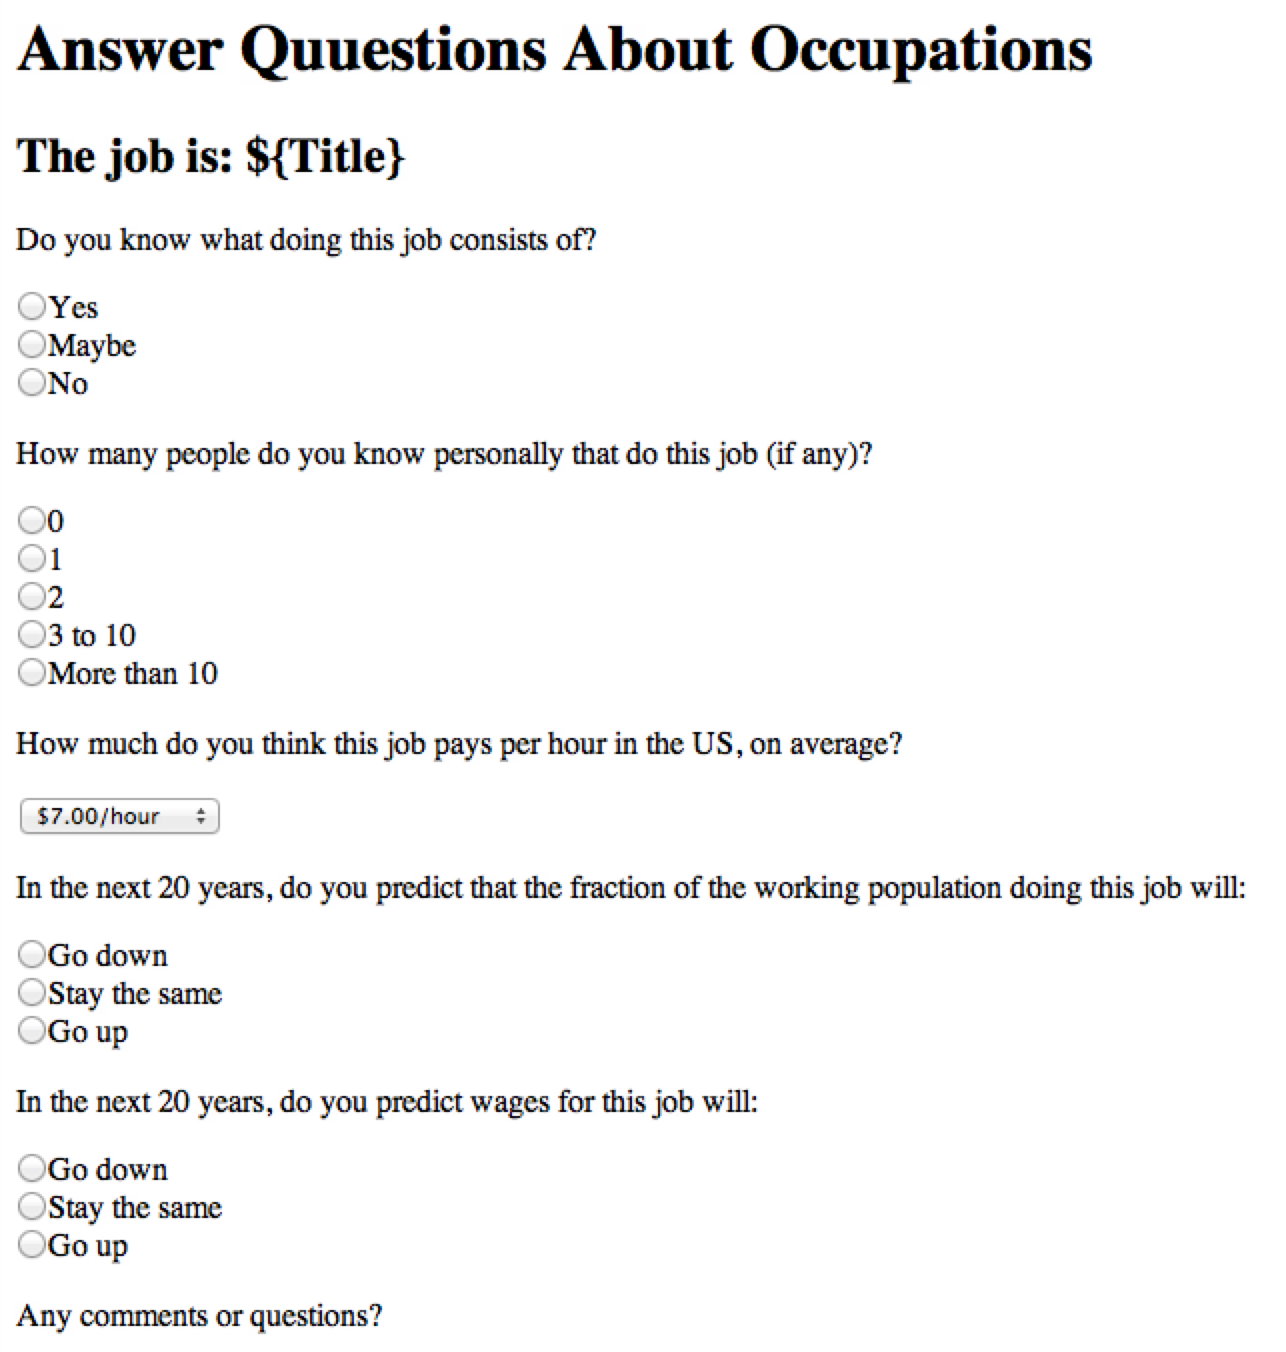
\includegraphics[width = \linewidth]{./images/survey.png}
\end{minipage}  
\end{figure} 

\section{Occupational knowledge} 
In Figure~\ref{fig:knowledge_by_occupation}, we plot the mean knowledge index by occupations.  

\begin{figure}
\caption{General Knowledge Index by BLS occupation title \label{fig:knowledge_by_occupation}} 
\centering
\begin{minipage}{0.95 \linewidth}
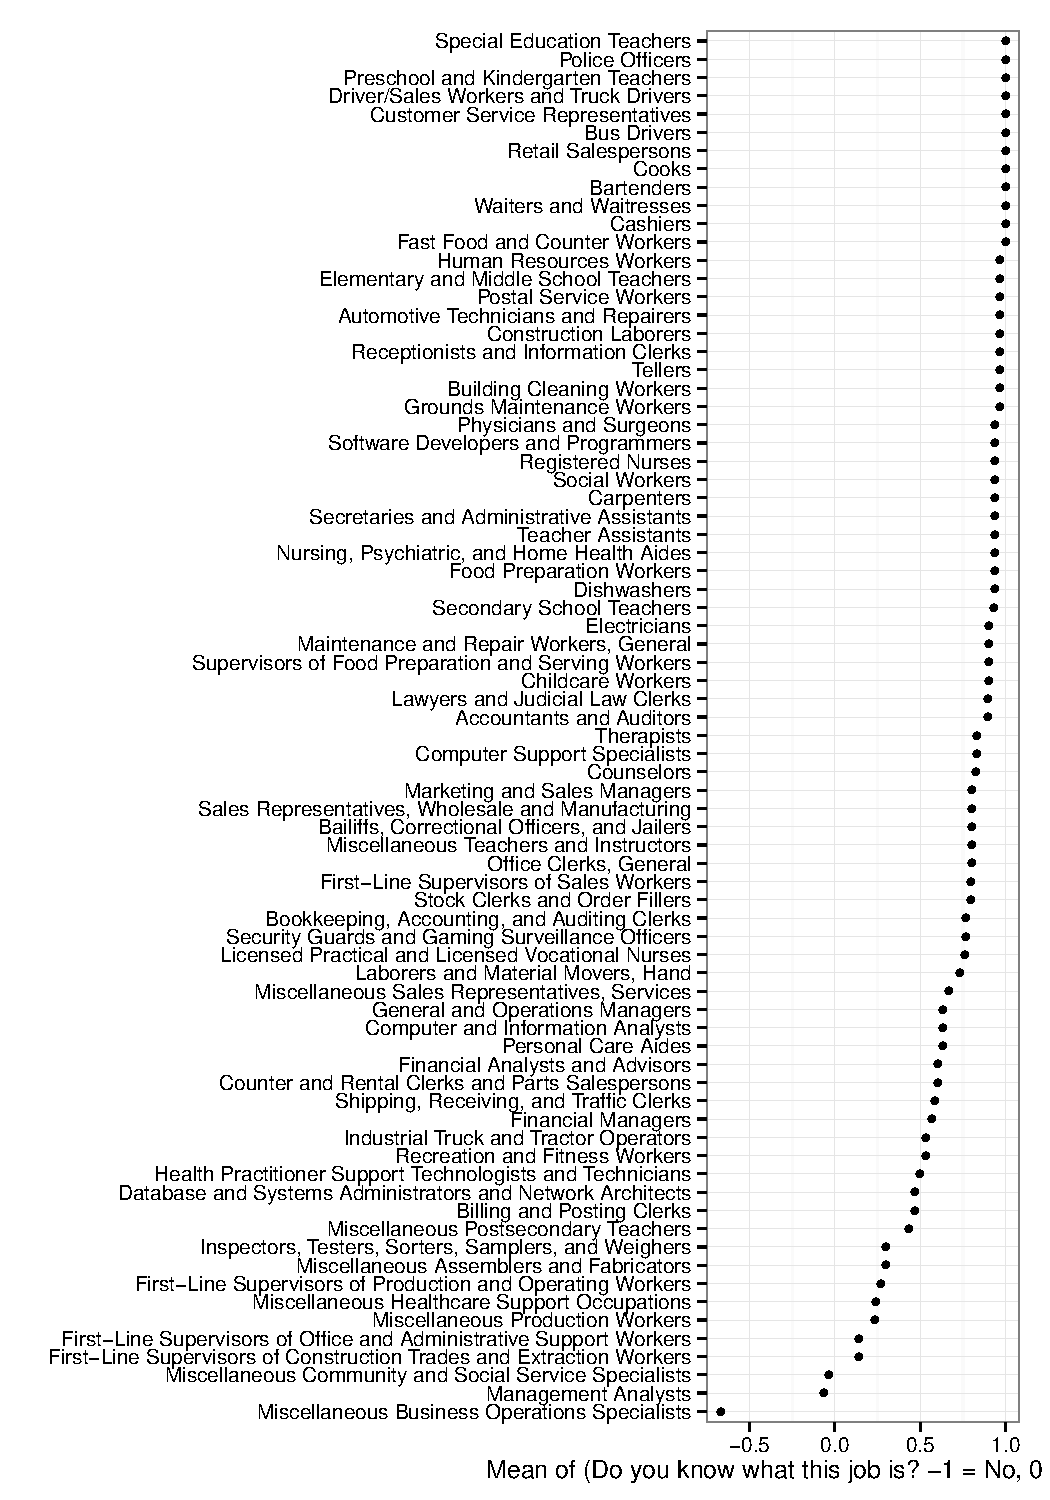
\includegraphics[width = \linewidth]{./plots/knowledge_by_occupation.pdf}
\end{minipage}  
\end{figure} 

\begin{figure}
\caption{Social Knowledge Index by BLS occupation title} \label{fig:social_by_occupation}  
\centering
\begin{minipage}{0.95 \linewidth}
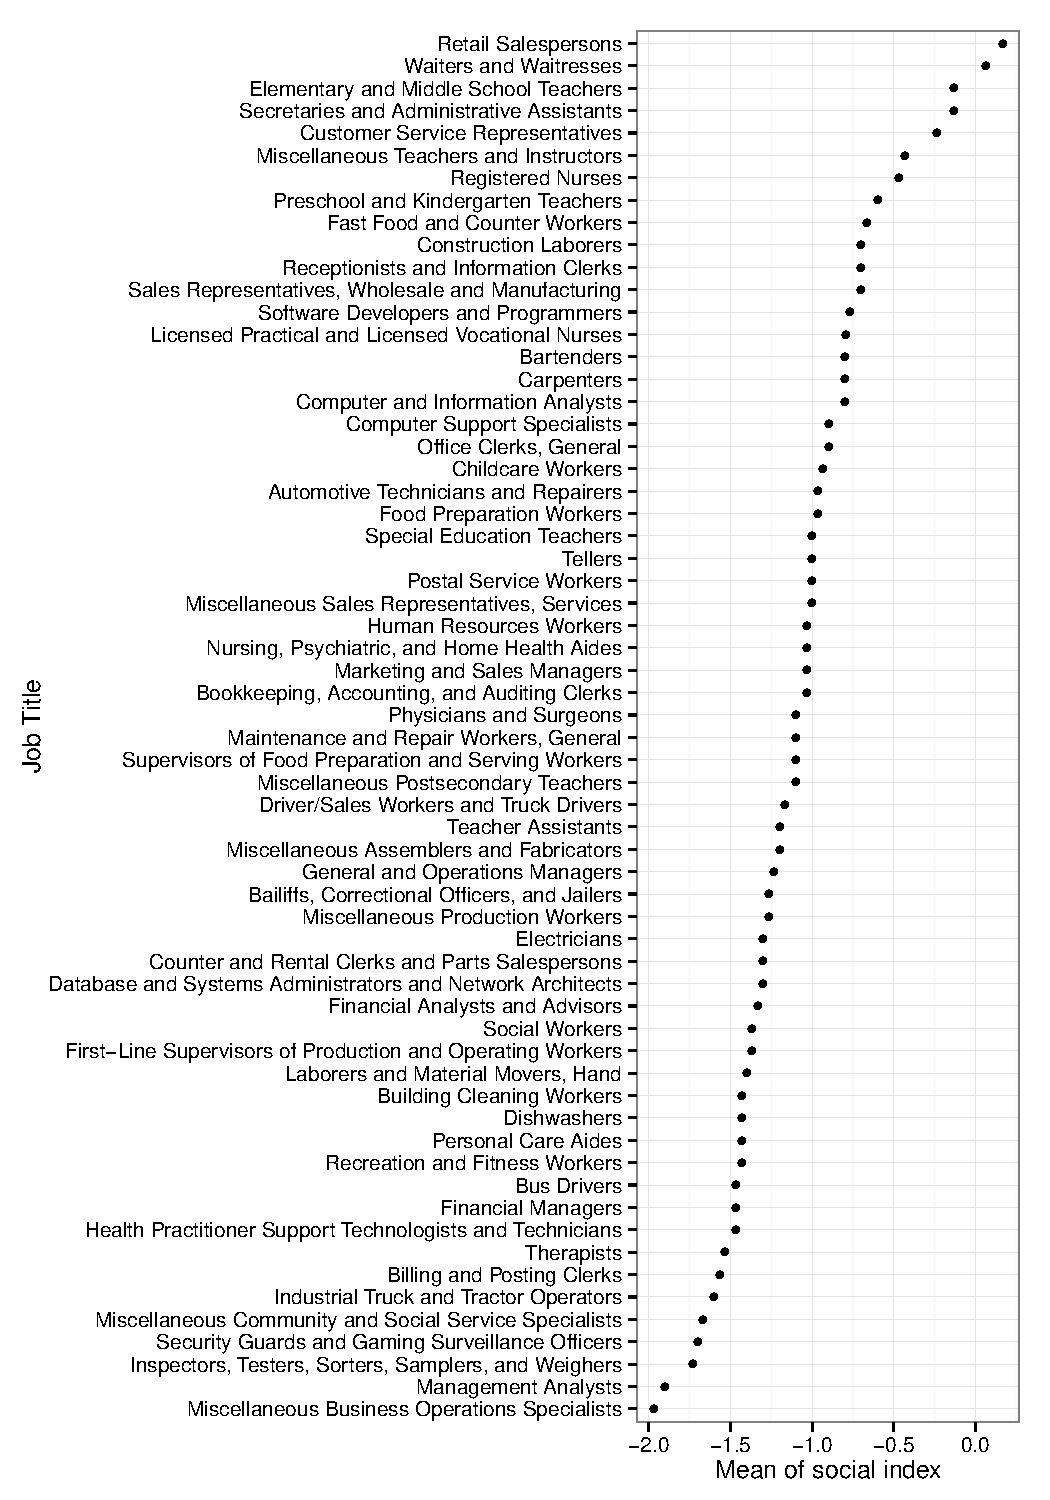
\includegraphics[width = \linewidth]{./plots/social_by_occupation.pdf}
\end{minipage}  
\end{figure} 

 [1] "OCC_CODE"       "OCC_TITLE"      "OCC_GROUP"      "TOT_EMP"       
 [5] "EMP_PRSE"       "H_MEAN"         "A_MEAN"         "MEAN_PRSE"     
 [9] "H_PCT10"        "H_PCT25"        "H_MEDIAN"       "H_PCT75"       
[13] "H_PCT90"        "A_PCT10"        "A_PCT25"        "A_MEDIAN"      
[17] "A_PCT75"        "A_PCT90"        "ANNUAL"         "HOURLY"        
[21] "imputed.hourly"
 [1] "title"               "know.job"            "social.knowledge"   
 [4] "predicted.wage"      "Answer.volume_trend" "Answer.wage_trend"  
 [7] "Answer.comment"      "WorkerId"            "know"               
[10] "social"              "v.trend"             "w.trend"            


\end{document} 
